\documentclass[german,a5paper, twoside]{scrreprt} %report veraltet, scrreprt neu
%Packages
\usepackage{geometry} %Definition Satzspiegel
\geometry{left=1.3cm,right=1.3cm,top=1.2cm,bottom=1.3cm} 
\usepackage[ngerman]{babel}%auch für Umlaute???
\usepackage{bibgerm}%deutsche trennung
\usepackage[utf8]{inputenc}%Zeichensatz
\usepackage[T1]{fontenc}%fontsatz
\usepackage{geometry}
\geometry{a5paper}
\usepackage{setspace} 
\usepackage{musixtex} 
\usepackage{musixguit}
\usepackage{graphicx} %Graphiken
\usepackage{float}
\usepackage{placeins}
\usepackage{pdfpages}%mehrseitige PDFs einbinden
\usepackage{fancyhdr}%Kopfzeilen usw.
\usepackage{tikz}

\newcommand{\chort}[2]{\chord{\textbf{#1}}{#2}}
%\newcommand{\Liedname}{Fruehlingserwachen}
%\newcommand{\Abstand}{5mm}

\newcommand{\Liedname}{Trolltraeume}
\newcommand{\Abstand}{4.5cm} %statt der 5cm einfach einen Abstand eingeben, damit der Text nicht mehr über den Noten ist. Faustregel: ungefähr 1.25cm pro Notenzeile

\newcommand{\Lizenz}{CC-BY-SA} %ist Standardmäßig eine CC4.0-BY-SA Lizenz. Wenn das nicht gewollt ist, CC-BY-SA einfach entfernen.



\usepackage{hyperref}

\begin{document}
\pagestyle{empty}
\begin{tikzpicture}[remember picture,overlay]
\node[anchor=north west,inner sep=5pt] at (current page.north west)
{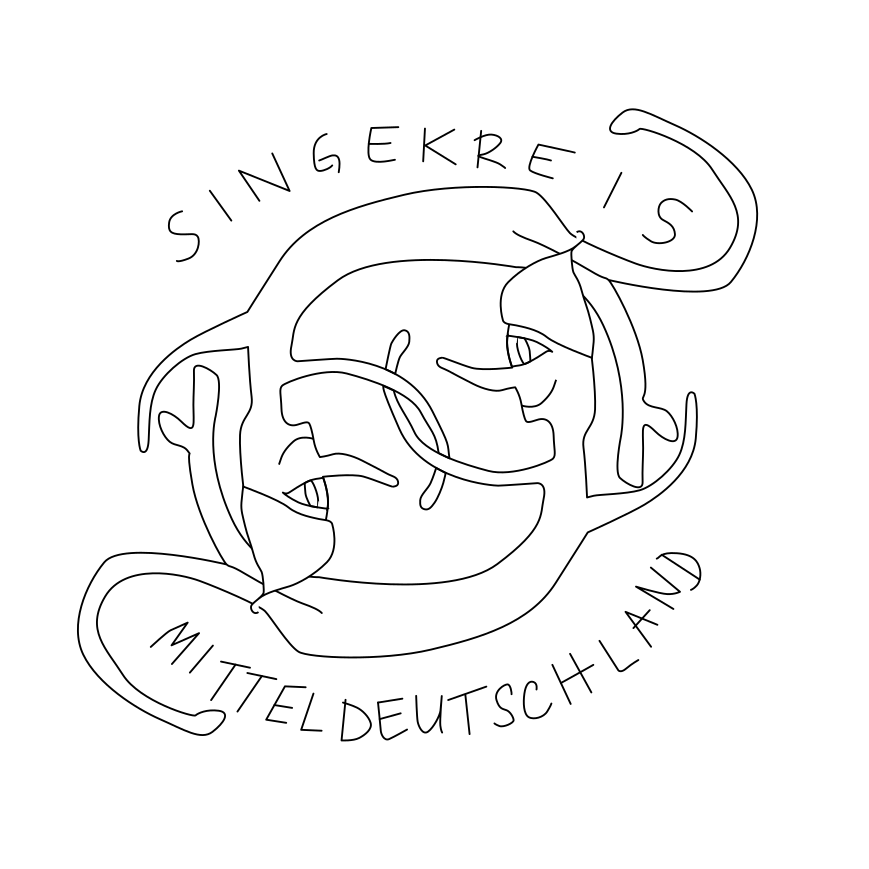
\includegraphics[width=.15\textwidth]{Rohdaten/Bilder/Singekreis.png}};
\end{tikzpicture} 
\ifthenelse{\equal{\Lizenz}{CC-BY-SA}}{
\begin{tikzpicture}[remember picture,overlay]
\node[anchor=south east,inner sep=5pt] at (current page.south east)
{
\includegraphics[width=.2\textwidth]{Rohdaten/Bilder/Lizenz.png}};
\end{tikzpicture} 
}{}

\begin{figure}[H]
\includepdf[trim=00mm 0mm 00mm 30mm ,pagecommand={},pages=1,width=1.1\textwidth]{Rohdaten/Noten/\Liedname _Noten.pdf}
\end{figure}
\vspace{\Abstand}

\begin{song} \noindent
%Hier kommen die Strophen rein. 
%für Akkorde: \chort{Akkord}{Wort über dem der Akkord stehen soll}
%Strophenzahl/Refrain: \textbf{Refrain:} 

%\textbf{2.}\chort{d}{Heißer} \chort{a}{Tee} und \chort{C}{Funken}\chort{F}{glut}

\textbf{2.}\chort{e}{Der} kleine Troll liegt \chort{G}{müd} im Bett und \chort{D}{träumt} er sei schon \chort{e}{12}.\\
Er will nun nur noch \chort{G}{tanzen} gehen, ins \chort{D}{Bett} gehen erst um \chort{e}{Ölf}.\\
Haus\chort{G}{aufgaben}, \chort{D}{Mathe} schwänzen, \chort{C}{Trollbier} \chort{D}{gibt’s} vom \chort{G}{Fass}.\\
\chort{e}{Visionen} haben, \chort{G}{Welt} verändern und \chort{e}{alle} \chort{D}{sagen}: \chort{e}{Lass} das!\\[0.3em]
\textbf{Ref.:} \chort{h}{Doch} kleine Trolle \chort{D}{tun} nicht gern, was \chort{A}{man} zu ihnen \chort{D}{sagt}.\\
Sie \chort{e}{singen}, tanzen, \chort{D}{springen} gern. Und \chort{A}{das} den \chort{H$^7$}{ganzen} \chort{e}{Tag}.\\[0.3em]
\textbf{3.} \chort{e}{Als} großer Troll hat \chort{G}{er} gelernt, dass \chort{D}{man} dies lieber \chort{e}{lässt}.\\
Er singt und tanzt und \chort{G}{springt} nicht gern, geht \chort{D}{nie}mals auf ein \chort{e}{Fest}.\\
Bau\chort{G}{sparverträge}, \chort{D}{keine} Zeit schaut \chort{C}{nie} zu \chort{D}{tief} ins \chort{G}{Glas} \\
und sei\chort{e}{nem} Kind, das \chort{G}{Spaß} nur hat, sagt \chort{e}{er} nur \chort{D}{ganz} streng: \chort{e}{Lass} das!\\[0.3em]
\textbf{4.} \chort{e}{Der} kleine Troll, der \chort{G}{wacht} nun auf, hat \chort{D}{Schweiß} noch im Ge\chort{e}{sicht}.\\
Was für ein Schrecken, \chort{G}{großer} Graus, so \chort{D}{werden} will ich \chort{e}{nicht}! \\
Drum \chort{G}{sing} und tanz und \chort{D}{spring} ich gern und \chort{C}{habe} \chort{D}{ganz} viel \chort{G}{Spaß}. \\
Und \chort{e}{wenn} ich einmal \chort{G}{Papa} bin will \chort{e}{ich} nicht \chort{D}{sagen}: \chort{e}{Lass} das!

\end{song}


\end{document}
